% Part 2 chapter carrying "Matter-Antimatter Asymmetry and the Information Writing Constraint" (March 2026), "The Baryon Asymmetry as a Derived
% Quantity: CMB Evidence Without BBN Prior" (March 2026) and the 18th-chain record, in that order. Read in full 2026-10-02 (438, 242, 7 lines,
% 50-line ledgers). Not carried (author 2026-10-02, speculation): 10^9 annihilation partners as the dark sector; weak force as
% 'force of becoming' / EW breaking as 'origin of duration'; '95 % memory, 5 % present'; CP phase fixed by the loop. Numbers: docs/verification/scripts/verify_cc_and_baryon.py. Checks: CC_AND_BARYON_CHECK.md (C3-C12, items 18-25).
\chapter{The baryon density}\label{ch:baryon}

\section{The size of the asymmetry}
One baryon survives for about $10^9$ photons: $\eta=(n_b-n_{\bar b})/n_\gamma\simeq6.1\times10^{-10}$, measured from the light-element
abundances (Big Bang nucleosynthesis)~\cite{Cyburt2016} and from the CMB acoustic peaks~\cite{Planck2018VI}, with the same value. \observed The Sakharov conditions~\cite{Sakharov1967} (baryon-number violation,
C and CP violation, departure from equilibrium) say how an asymmetry can arise; the CP violation of the CKM matrix~\cite{KobayashiMaskawa1973} is too small to give the
measured $\eta$~\cite{Gavela1994}, and electroweak baryogenesis~\cite{KuzminRubakovShaposhnikov1985}, leptogenesis~\cite{FukugitaYanagida1986} and Affleck--Dine models~\cite{AffleckDine1985} each leave $\eta$ set by parameters they do not derive.

\section{The question IAM asks}
At the cosmic horizon, a place in IAM, baryons write classical records on the horizon through gravitational decoherence, at $k_BT_{GH}\ln2$ per bit,
and the accumulated cost of that writing is
identified with $\Lambda$ (Chapter~\ref{ch:lambda}). The writing depends on the baryon density, which $\eta$ fixes. The proposal is a
self-consistency loop,
\begin{equation}\eta\to n_b\to\dot W_{\rm info}\to\Lambda\to H(a)\to\eta,\end{equation}
with the measured $\eta$ as its fixed point: the Sakharov dynamics generate an asymmetry, and the writing constraint selects its size. \conjecture\ The
loop does not derive $\eta$. A derivation needs: (1) the writing rate at the QCD transition, where the universe is
radiation dominated; (2) the horizon capacity there; (3) the link to the Sakharov mechanism. For scale at $T=150$\,MeV: $a\simeq9.6\times10^{-13}$,
$l_H\simeq15.5$\,km, and the horizon holds $2.9\times10^{78}$ Planck-area bits. \calc

\section{One relation, read as $\eta$}
Inverting the cosmological-constant expressions for $\Omega_bh^2$ at the Planck $\Omega_mh^2=0.1430$, with $\eta=273.9\times10^{-10}\,\Omega_bh^2$:
the baseline (with $2/\pi$, without $\sqrt{\Omega_\Lambda}$) gives $\eta=5.03\times10^{-10}$; with $\sqrt{\Omega_\Lambda}$ it gives
$6.08\times10^{-10}$, $0.5$--$0.9\,\%$ below the CMB values of the chains below ($6.113$--$6.137$). \calc This is the relation $\Omega_b/\Omega_m=(3/16)\sqrt{\Omega_\Lambda}$ of
Chapter~\ref{ch:lambda} in another variable. The cosmological constant and the baryon density are one measured relation, not two.
The derivation is written out step by step, with the status of each premise, in Appendix~\ref{app:der:lambda}.

\section{The 18th chain}

\begin{figure}[htbp]\centering
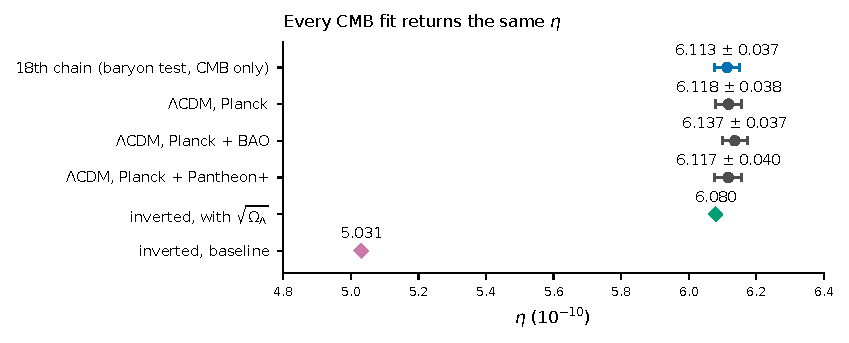
\includegraphics[width=0.75\textwidth]{figures/part2/fig_eta.pdf}
\caption{$\eta=273.9\times10^{-10}\,\Omega_bh^2$ on the 18th chain ($6.113\pm0.037$) and on the $\Lambda$CDM chains ($6.117$--$6.137$): every CMB fit returns the same baryon density \observed. Diamonds: the cosmological-constant expressions inverted for $\Omega_bh^2$ at $\Omega_mh^2=0.1430$, 6.080 with $\sqrt{\Omega_\Lambda}$ and 5.031 without; this is the relation of Fig.~\ref{fig:cc_relation} in another variable. \calc}\label{fig:eta}
\end{figure}
A Planck 2018 chain (MGCAMB~\cite{Zhao2009MGCAMB,Wang2023MGCAMB} with $\mu_0=-0.13495$ fixed; low-$\ell$ TT and EE, plik TTTEEE lite, lensing~\cite{Planck2018V,Planck2018VIII}) was run with
$\Omega_bh^2$ sampled over a flat range $[0.010,0.040]$, six times wider than the $[0.020,0.025]$ of the other runs. No light-element abundance
data enter. Helium is set inside CAMB~\cite{Lewis2000CAMB} from $\Omega_bh^2$ by its standard nucleosynthesis relation, which affects only the damping tail.
The chain ran 19--20 March 2026 to 22,400 accepted steps, $R-1=0.009273$. With 30\,\% burn-in (14,957 rows):
\begin{equation}\Omega_bh^2=0.02232\pm0.00014,\qquad\eta=(6.113\pm0.037)\times10^{-10},\qquad
\frac{\Omega_b/\Omega_m}{(3/16)\sqrt{\Omega_\Lambda}}=1.0046\pm0.0068 .\end{equation}
\fitted
The $\Lambda$CDM chains in the same repository return the same $\eta$: $6.118$ (Planck), $6.137$ (Planck + BAO), $6.117$ (Planck + Pantheon+).
\begin{table}[htbp]\centering\small
\caption[The baryon density on every chain]{The baryon density on every chain, $\eta=273.9\times10^{-10}\,\Omega_bh^2$ (30\,\% burn-in, weighted mean and standard deviation; rows after burn-in), and the cosmological-constant expressions inverted for $\Omega_bh^2$ at the Planck $\Omega_mh^2=0.1430$.}\label{tab:baryon_chains}
\begin{adjustbox}{max width=\textwidth}
\begin{tabular}{lcrccll}\toprule
Source & $\Omega_bh^2$ range & rows & $\Omega_bh^2$ & $10^{10}\eta$ & ratio to $(3/16)\sqrt{\Omega_\Lambda}$ & Label\\\midrule
18th chain (CMB only) & 0.010--0.040 & 14{,}957 & $0.02232\pm0.00014$ & $6.113\pm0.037$ & $1.0046\pm0.0068$ & \measured\\
$\Lambda$CDM, Planck & 0.020--0.025 & 12{,}544 & $0.02234\pm0.00014$ & $6.118\pm0.038$ & $1.0058\pm0.0067$ & \measured\\
$\Lambda$CDM, Planck + BAO & 0.020--0.025 & 12{,}600 & $0.02240\pm0.00014$ & $6.137\pm0.037$ & $1.0106\pm0.0064$ & \measured\\
$\Lambda$CDM, Planck + Pantheon+ & 0.020--0.025 & 21{,}168 & $0.02233\pm0.00014$ & $6.117\pm0.040$ & $1.0056\pm0.0070$ & \measured\\
Expression with $2/\pi$, without $\sqrt{\Omega_\Lambda}$ & --- & --- & $0.01837$ & $5.031$ & --- & \calc\\
Expression with $\sqrt{\Omega_\Lambda}$ & --- & --- & $0.02220$ & $6.080$ & --- & \calc\\\bottomrule
\end{tabular}
\end{adjustbox}
\end{table}
They must. The informational term is off at recombination ($E\to0$), so the early universe is $\Lambda$CDM and the acoustic peaks measure the same
baryon density with or without it. The chain is the consistency check that the term leaves the early universe intact, and it passes.
The CMB measures $\Omega_bh^2$ from the relative heights of the acoustic peaks; the chain does this measurement, as every Planck fit does, and its
agreement with nucleosynthesis is the established CMB--BBN concordance~\cite{Cyburt2016}. The chain contains no IAM constraint on $\Omega_b$: the writing
constraint is not in its likelihood, and fixing $\mu_0$ or widening the range does not move $\Omega_bh^2$. What the chain adds is the
relation of Chapter~\ref{ch:lambda} evaluated on a CMB-only posterior: $0.7\sigma$.
\begin{figure}[htbp]\centering
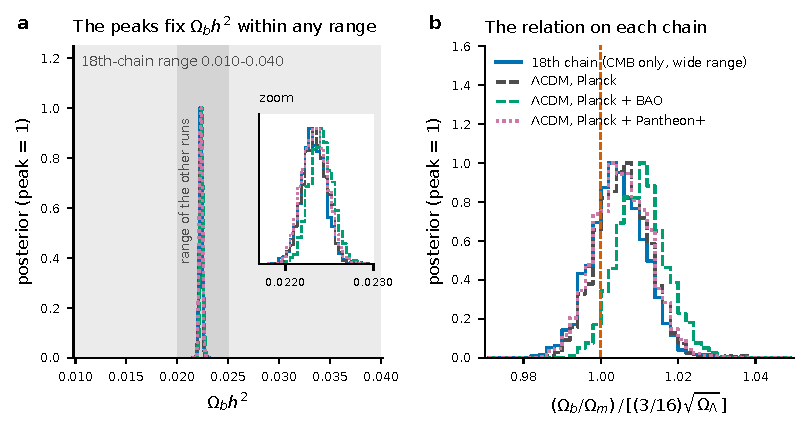
\includegraphics[width=\textwidth]{figures/part2/fig_baryon_posterior.pdf}
\caption[The 18th chain against the $\Lambda$CDM chains]{(a) The $\Omega_bh^2$ posterior of the 18th chain, sampled over the flat range 0.010--0.040 (light band; the darker band is the 0.020--0.025 of the other runs), and of the three $\Lambda$CDM chains; inset: the peaks enlarged. The acoustic peaks fix $\Omega_bh^2=0.02232\pm0.00014$ whatever the range. (b) The posterior of $(\Omega_b/\Omega_m)/[(3/16)\sqrt{\Omega_\Lambda}]$ on the same chains. Chain files in \texttt{mgcamb\_validation/\allowbreak{}chains}, 30\,\% burn-in, weighted. \measured}\label{fig:baryon_posterior}
\end{figure}

Before the chain was run, the expectation was that a chain with $\Omega_bh^2$ free would return $\eta\simeq6\times10^{-10}$. Because the early universe is unchanged,
every CMB fit returns that value; the chain confirms consistency, not selection. The test of selection is a chain in which the writing constraint itself is in the
likelihood, so that $\Omega_b$ is predicted from $\Lambda$ rather than measured from the peaks. \openprob

\section{What would make it a derivation}
(1) $3/16$ from physics, with the geometric factor and the $\sqrt{\Omega_\Lambda}$ fixed before the comparison; (2) the writing rate and
horizon capacity at the QCD transition, which the loop requires and which are not yet formulated; (3) the reason the relation holds today and
not at other epochs. Chapter~\ref{ch:lambda} shows that heat radiated by baryons is not the measure of the cost ($3\times10^{-8}$ of $\rho_\Lambda$); a
derivation must work in the horizon-entropy variable carried by $\beta_mE(a)$, priced by IAM's Law at $k_BT_{GH}\ln2$ per bit, with the virial half setting how much bound matter writes. \openprob
